\section{Start Using Thunderbird}

\begin{figure}[htbp]
\centering

\includegraphics{thunderbird.jpg}
\caption{Thunderbird}
\end{figure}

In upcoming sections, we will be using Mozilla's Thunderbird e-mail
program to show you how to configure your e-mail client for maximum
security. Similar to Mozilla's Firefox browser, Thunderbird has many
security advantages over its counterparts like Apple Mail and Outlook.

Thunderbird is a so-called ``mail user agent'' (MUA). This is different
from web-based e-mail services like Google's Gmail. You must install the
Thunderbird application on your computer. Thunderbird has a nice
interface and features that enable you to manage multiple mailboxes,
organize messages into folders, and search through mails easily.

Thunderbird can be configured to work with your existing e-mail account,
whether that account is through your Internet Service Provider (such as
Comcast) or through an web-based email provider (such as Gmail).

Using Thunderbird has many advantages over using web-based e-mail
interfaces. These will be discussed in the following chapter. To
summarize, though, Thunderbird enables much greater privacy and security
than web-based e-mail services.

This section provides information on how to install Thunderbird on
Windows, Mac OS X, and Ubuntu.

\subsection{Installing Thunderbird on Windows}

Installing Thunderbird involves two steps: first, download the software
and then run the installation program.

\begin{enumerate}[1.]
\item
  Use your web browser to visit the Thunderbird download page at
  \href{http://www.mozillamessaging.com/en-US/thunderbird/}{http://www.mozillamessaging.com/en-US/thunderbird/}.
  This page detects your computer's operating system and language, and
  recommends the best version of Thunderbird for you to use.
\end{enumerate}
\begin{figure}[htbp]
\centering
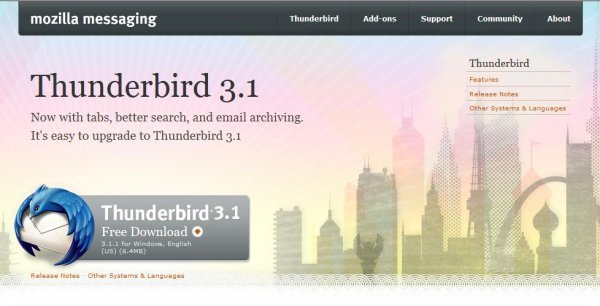
\includegraphics{thunderbird_inst_1.jpg}
\caption{Thunderbird Install}
\end{figure}

If you want to use Thunderbird in a different language or with a
different operating system, click the \emph{Other Systems and Languages}
link on the right side of the page and select the version that you need.

\begin{enumerate}[1.]
\setcounter{enumi}{1}
\item
  Click the download button to save the installation program to your
  computer.
\end{enumerate}
\begin{figure}[htbp]
\centering
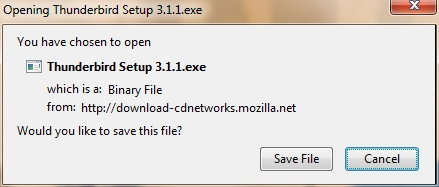
\includegraphics{thunderbird_inst_2.jpg}
\caption{Thunderbird Install}
\end{figure}

Click the \textbf{Save} button to save the Thunderbird Setup file to
your computer.

\begin{enumerate}[1.]
\setcounter{enumi}{2}
\item
  Close all applications running on your computer.
\item
  Find the setup file on your computer (it's usually in the Downloads
  folder or on your desktop) and then double-click it to start the
  installation. The first thing that the installer does is display the
  \textbf{Welcome to the Mozilla Thunderbird Setup Wizard} screen.
\end{enumerate}
\begin{figure}[htbp]
\centering
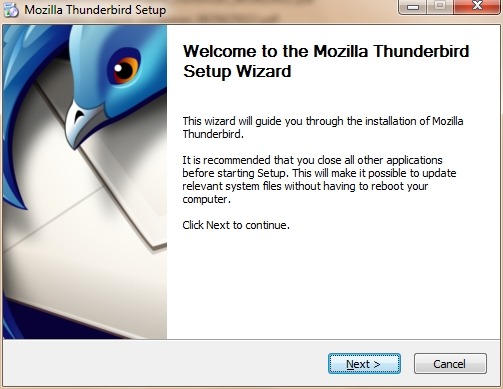
\includegraphics{thunderbird_inst_3.jpg}
\caption{Thunderbird Install}
\end{figure}

Click the \textbf{Next} button to start the installation. If you want to
cancel it, click the \textbf{Cancel} button.

\begin{enumerate}[1.]
\setcounter{enumi}{4}
\item
  The next thing that you see is the \textbf{Setup Type} screen. For
  most users the Standard setup option is good enough for their needs.
  The Custom setup option is recommended for experienced users only.
  Note that Thunderbird installs itself as your default mail
  application. If you do not want this, clear the checkbox labeled
  \textbf{Use Thunderbird as my default mail application}.
\end{enumerate}
\begin{figure}[htbp]
\centering
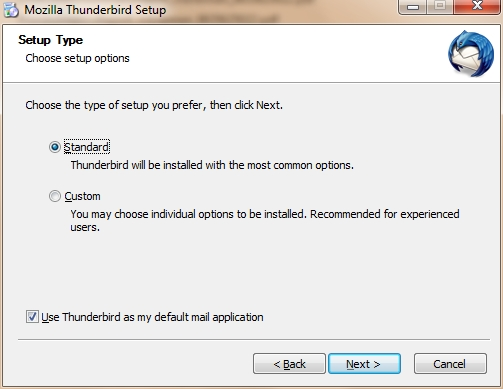
\includegraphics{thunderbird_inst_4.jpg}
\caption{Thunderbird Install}
\end{figure}

Click the \textbf{Next} button to continue the installation.

\begin{enumerate}[1.]
\setcounter{enumi}{5}
\item
  After Thunderbird has been installed, click the \textbf{Finish} button
  to close the setup wizard.
\end{enumerate}
\begin{figure}[htbp]
\centering
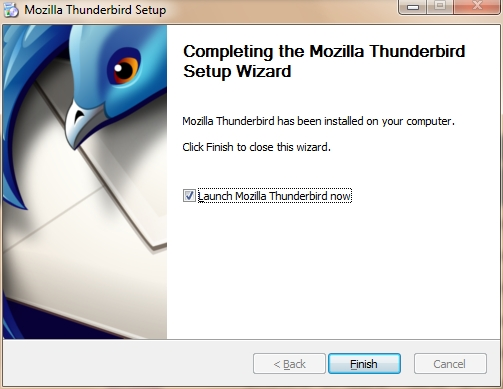
\includegraphics{thunderbird_inst_5.jpg}
\caption{Thunderbird Install}
\end{figure}

If the \textbf{Launch Mozilla Thunderbird} now checkbox is selected,
Thunderbird starts after it has been installed.

\subsection{Installing Thunderbird on Ubuntu}

There are two different procedures for installing Thunderbird on Ubuntu:
one for version 10.04 or later, and one for earlier versions of Ubuntu.
We describe both below.

Thunderbird will not run without the following libraries or packages
installed on your computer:

\begin{itemize}
\item
  GTK+ 2.10 or higher
\item
  GLib 2.12 or higher
\item
  Pango 1.14 or higher
\item
  X.Org 1.0 or higher
\end{itemize}
Mozilla recommends that a Linux system also has the following libraries
or packages installed:

\begin{itemize}
\item
  NetworkManager 0.7 or higher
\item
  DBus 1.0 or higher
\item
  HAL 0.5.8 or higher
\item
  GNOME 2.16 or higher
\end{itemize}
\subsection{Installing Thunderbird on Ubuntu 12.04 or newer}

If you're using Ubuntu 12.04 or newer, the easiest way to install
Thunderbird is through the Ubuntu Software Center.

\begin{enumerate}[1.]
\item
  Type Software in the Untiy search window.
\end{enumerate}
\begin{figure}[htbp]
\centering
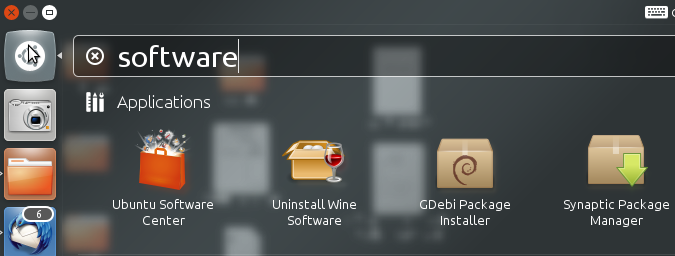
\includegraphics{thunderbird_inst_ubuntu_1.jpg}
\caption{Thunderbird Install}
\end{figure}

\begin{enumerate}[1.]
\setcounter{enumi}{1}
\item
  Click on `Ubuntu Software Center'
\item
  Type ``Thunderbird'' in the search box and press the Enter on your
  keyboard. The Ubuntu Software Center finds Thunderbird in its list of
  available software.
\item
  Click the \textbf{Install} button. If Thunderbird needs any additional
  libraries, the Ubuntu Software Center alerts you and installs them
  along with Thunderbird.
\end{enumerate}
You can find the shortcut to start Thunderbird in the Internet option
under the Applications menu:

\begin{figure}[htbp]
\centering
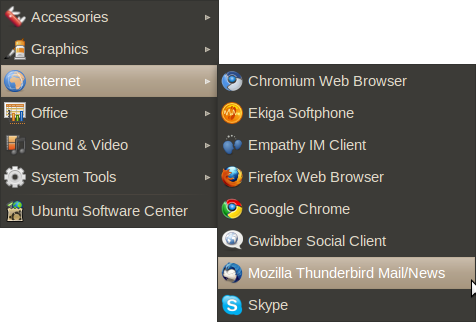
\includegraphics{thunderbird_inst_ubuntu_2.jpg}
\caption{Thunderbird Install}
\end{figure}

\subsection{Installing Thunderbird on Mac OS X}

To install Thunderbird on your Mac, follow these steps:

\begin{enumerate}[1.]
\item
  Use your web browser to visit the Thunderbird download page at
  \href{http://www.mozillamessaging.com/en-US/thunderbird/}{http://www.mozillamessaging.com/en-US/thunderbird/}.
  This page detects your computer's operating system and language, and
  it recommends the best version of Thunderbird for you to use.
\end{enumerate}
\begin{figure}[htbp]
\centering
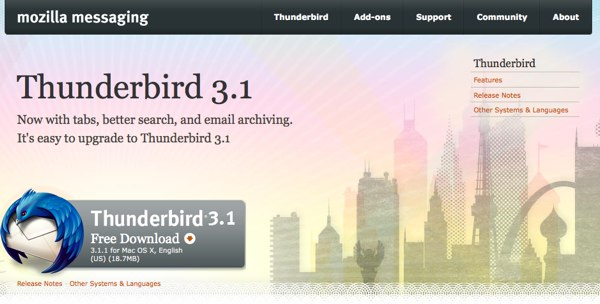
\includegraphics{thunderbird_inst_mac_1.jpg}
\caption{Thunderbird Install}
\end{figure}

\begin{enumerate}[1.]
\setcounter{enumi}{1}
\item
  Download the Thunderbird disk image. When the download is complete,
  the disk image may automatically open and mount a new volume called
  \emph{Thunderbird}.
\end{enumerate}
If the volume did not mount automatically, open the Download folder and
double-click the disk image to mount it. A Finder window appears:

\begin{figure}[htbp]
\centering
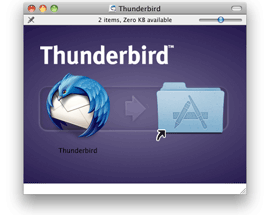
\includegraphics{thunderbird_inst_mac_2.jpg}
\caption{Thunderbird Install}
\end{figure}

\begin{enumerate}[1.]
\setcounter{enumi}{2}
\item
  Drag the Thunderbird icon into your Applications folder. You've
  installed Thunderbird!
\item
  Optionally, drag the Thunderbird icon from the Applications folder
  into the Dock. Choosing the Thunderbird icon from the Dock lets you
  quickly open Thunderbird from there.
\end{enumerate}
\begin{figure}[htbp]
\centering
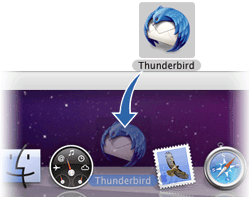
\includegraphics{thunderbird_inst_mac_3.jpg}
\caption{Thunderbird Install}
\end{figure}

\textbf{Note:} When you run Thunderbird for the first time, newer
versions of Mac OS X (10.5 or later) will warn you that the application
Thunderbird.app was downloaded from the Internet.

If you downloaded Thunderbird from the Mozilla site, click the
\textbf{Open} button.

\begin{figure}[htbp]
\centering
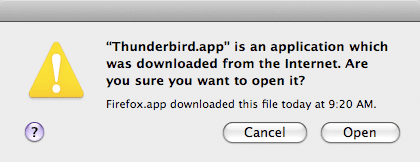
\includegraphics{thunderbird_inst_mac_4.jpg}
\caption{Thunderbird Install}
\end{figure}

\subsection{Starting Thunderbird for the first time}

After you have installed Thunderbird for the first time you will be
guided through the configuration of your mail account. These settings
are defined by your e-mail provider (your Internet Service Provider or
web-based e-mail service provider). The next chapter describes how to
set up your account and configure it for maximum security.
